% Shared preamble for the English summaries in this repository.
\documentclass[11pt,a4paper]{article}
\usepackage[margin=2.2cm]{geometry}
\usepackage[T1]{fontenc}
\usepackage[utf8]{inputenc}
\usepackage{lmodern}
\usepackage{amsmath,amssymb}
\usepackage{graphicx}
\usepackage{booktabs}
\usepackage{enumitem}
\usepackage[hidelinks]{hyperref}
\setlist{itemsep=2pt,topsep=4pt}
\setlength{\parindent}{0pt}
\setlength{\parskip}{5pt}
\graphicspath{{figures/}}
\newcommand{\summaryheader}[3]{%
  \begin{center}
    {\Large\bfseries #2}\\[3pt]
    {\large #1}\\[3pt]
    {\small Arshia Goshtasbi \textbullet{} MSc Electrical Engineering (Control), Iran University of Science and Technology \textbullet{} #3}
  \end{center}
  \vspace{2pt}\hrule\vspace{8pt}\par}

\begin{document}
\summaryheader{Reinforcement Learning, Course Project (with Kimia Aghili)}{Model-Free RL for the Fully Cooperative Consensus of Multi-Agent Systems}{Autumn 1403 (2024); code rewritten Aban 1405}

\section*{Problem}
We reproduced H.~Wang and M.~Li, ``Model-free reinforcement learning for fully cooperative consensus problem of nonlinear multiagent systems,'' \emph{IEEE TNNLS}, 2020. $N$ agents $\dot x_i=f(x_i)+g(x_i)u_i$ communicate over a directed graph with weights $e_{ij}$, in-degrees $d_i$ and Laplacian $L$. With the local neighbourhood errors $\delta_i=\sum_j e_{ij}(x_i-x_j)$, i.e.\ $\delta=(L\otimes I_n)x$, all agents minimise one shared cost
\[
J=\int_0^\infty \tfrac12 Q(\delta)+\tfrac12\textstyle\sum_i u_i^\top R_iu_i\,dt .
\]
Minimising the Hamiltonian gives $u_i^*=-d_iR_i^{-1}g_i^\top\partial V^*/\partial\delta_i+\sum_j e_{ji}R_i^{-1}g_i^\top\partial V^*/\partial\delta_j$: agent $i$ needs its own error and the errors of the agents that listen to it.

\section*{Off-policy integral Bellman equation}
Data are generated once with an exploring input $u$. For target policies $u_i^k$, the paper's eq.~(20) is
\[
V^{k+1}(\delta(t))-V^{k+1}(\delta(t{+}T))=\int_t^{t+T}\!\Big[\tfrac12Q(\delta)+\tfrac12\sum_i (u_i^k)^\top R_iu_i^k\Big]d\tau+\int_t^{t+T}\sum_i(u_i^{k+1})^\top R_i(u_i-u_i^k)\,d\tau,
\]
which holds without knowing $f$ or $g$. With $V^{k+1}=W_c^\top\phi(\delta)$ and $u_i^{k+1}=W_{ai}^\top\psi_i$ it is linear in all weights. I solve it by least squares over 3{,}600 intervals of $T=0.05$\,s at each policy-iteration step (Algorithm~3), starting from the admissible $u^0=0$. Because $\delta$ lies in a subspace (the rows of $L$ are dependent), some basis columns are collinear and the minimum-norm solution is used.

\section*{Results}
\begin{center}
\begin{tabular}{lcccc}\toprule
Example & consensus & $\hat V(\delta(0))$ & $J$ & gap\\\midrule
Linear check (5 agents) & 6.2 s & 1.3398 & 1.3245 & 1.2\%\\
5 nonlinear agents (paper V-A.1) & 6.5 s & 0.4509 & 0.4501 & 0.18\%\\
20 nonlinear agents (paper V-A.2) & 7.5 s & 5.3070 & 5.2529 & 1.0\%\\\bottomrule
\end{tabular}
\end{center}
The paper reports consensus after about 6\,s and 8\,s with gaps of 0.83\% and 0.29\%. In the linear check the centralised Riccati equation gives $V^*=1.3233$, so the learned distributed controller is within 0.1\% of the best centralised one; the 1\% critic gap comes from the distributed actor structure. In both nonlinear examples the agents are stable on their own and $R_i$ is large (10 and 200), so the optimal input is small and $J$ is close to the cost with $u=0$ (0.4520 and 5.2573).

\begin{center}
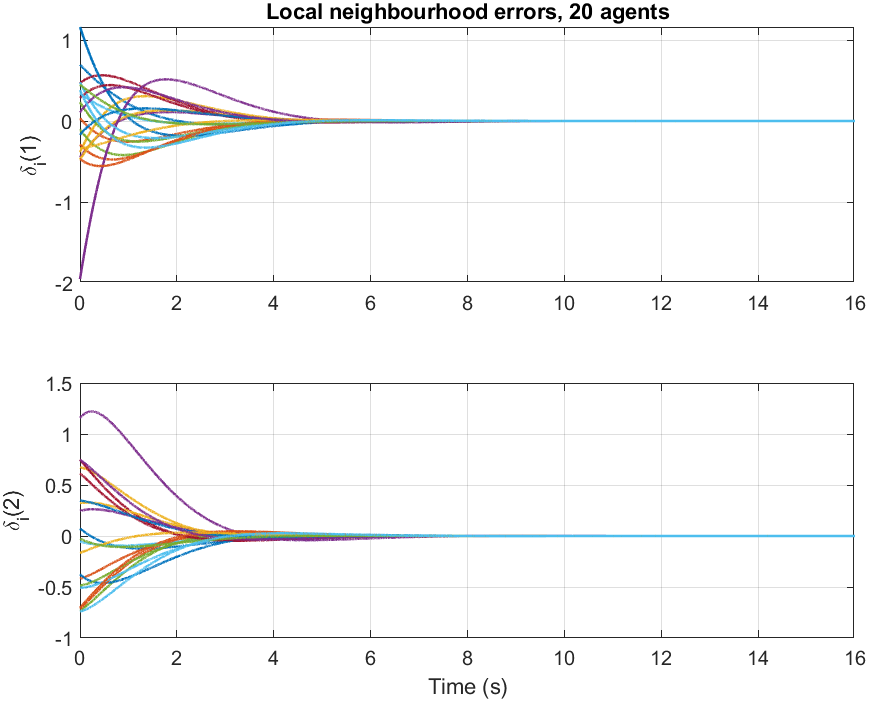
\includegraphics[width=0.52\textwidth]{twenty_errors.png}\hfill
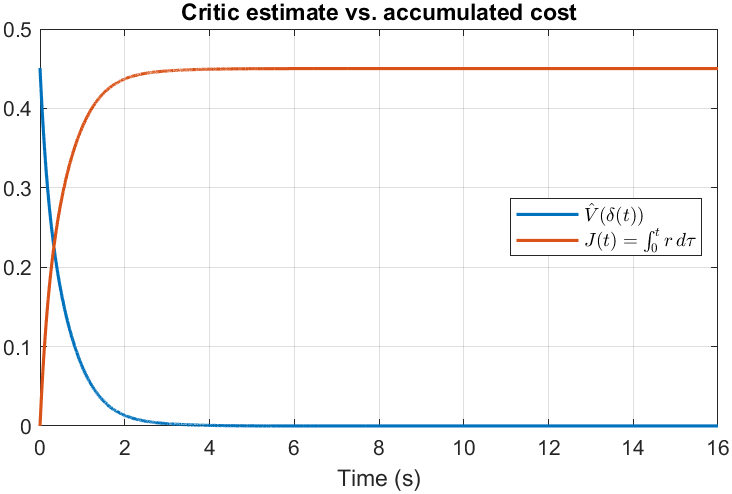
\includegraphics[width=0.45\textwidth]{five_value.png}
\end{center}

\section*{Choices not fixed by the paper}
The paper gives neither initial states nor activation functions. I used quadratic monomials of $\delta$ for the critic (plus quartic terms when $Q$ is quartic), each agent's error and its listeners' errors for the actor, plus a copy scaled by $\sin x_{i1}$, the agent's own input gain. The exploring input is a sum of six sinusoids per agent.
\end{document}
